\subsection{Assignment: An imaging problem}
Consider the following imaging problem (see Fig. 1): 3 light emitters ($E_j,\ j\in [1,3]$) are
positioned in known locations in a room. In order to find the power emanating from the
emitters, 4 detectors ($D_i,\ i\in[1,4]$) are positioned at certain locations. The power $I_d$ measured by the $i$-th detector is given by:
\begin{align}
    I_{d,i}\ &=\ \sum_{j=0}^{N}\frac{I_{e,j}}{\mathopen|r_{ij}\mathclose|^2},\\
    r_{ij}\ &=\ \sqrt{(D_i\ -\ E_j)^2}\\
    \mathrm{Imaging\ Forward\ Problem: }\ \mathbf{A I_e} &= \mathbf{I_d}\\
    \mathrm{Imaging\ Inverse\ Problem: }\ \mathbf{I_e} &= \mathbf{A^{-1} I_d}\\  
\end{align}
where I$_{e,j}$ is the power of the $j$-th intensity source and r$_{ij}$ is the Distance between the detector and emitter.



\subsubsection{Build the matrix for the imaging problem defined above}
\begin{lstlisting}
%% Assignment 2 An imaging problem
% a
s.orig.D = [-1,1;1,1;1,-1;-1,-1];
s.orig.E = [-0.5,0.5;0,0;0.5,0.5];
s.orig.I_e = [4,3,1];
s.orig.A = zeros(length(s.orig.D),length(s.orig.E));

for i = 1:length(s.orig.D)
    for j = 1:length(s.orig.E)
        s.orig.A(i,j) = 1./sqrt(sum((s.orig.D(i,:)-s.orig.E(j,:)).^2));
    end
end
\end{lstlisting}




\subsubsection{What are the detected values for the source values [$\mathbf{I_{e,1}, I_{e,2}, I_{e,3}}$] = [$\mathbf{4, 3, 1}$]?
Consider these detected values as the measured data.}
\begin{lstlisting}
%% b
s.orig.I_d = s.orig.A * s.orig.I_e';
\end{lstlisting}

\begin{align}
\mathbf{A}\ &=\ \left(\begin{array}{ccc} \sqrt{2} & \frac{\sqrt{2}}{2} & \frac{\sqrt{2}\,\sqrt{5}}{5}\\ \frac{\sqrt{2}\,\sqrt{5}}{5} & \frac{\sqrt{2}}{2} & \sqrt{2}\\ \frac{\sqrt{2}}{3} & \frac{\sqrt{2}}{2} & \frac{\sqrt{2}\,\sqrt{5}}{5}\\ \frac{\sqrt{2}\,\sqrt{5}}{5} & \frac{\sqrt{2}}{2} & \frac{\sqrt{2}}{3} \end{array}\right)\\
\mathbf{I_d}\ &=\ \left(\begin{array}{c} 8.411\\ 6.065\\ 4.639\\ 5.123 \end{array}\right)
\end{align}




\clearpage
\subsubsection{Calculate the solution of the inverse problem based on the pseudo‐inverse of the
matrix}
\begin{lstlisting}
%% c
tol = 1e-5;
[s.orig.moore.I_e, s.orig.moore.A_inv] = SolPseudoInvMoore(s.orig.A,s.orig.I_d,tol);
\end{lstlisting}
\begin{lstlisting}
function [I_e_moore,A_inv_moore] = SolPseudoInvMoore(A,b,tol)
A_inv_moore = pinv(A,tol);
I_e_moore = A_inv_moore * b;
end
\end{lstlisting}
\begin{align}
    \mathbf{A_{inv,moore}}\ &=\ \left(\begin{array}{cccc} 1.144 & -0.08321 & -0.6567 & -0.4039\\ -0.8279 & -0.8279 & 1.535 & 1.535\\ -0.08321 & 1.144 & -0.4039 & -0.6567 \end{array}\right)\\
    \mathbf{I_{e,moore}}\ &=\ \left(\begin{array}{c} 4.0\\ 3.0\\ 1.0 \end{array}\right)
\end{align}



\clearpage
\subsubsection{ Calculate the solution of the inverse problem based on the singular value
decomposition (SVD) of the matrix}
\begin{align}
    \mathbf{A_{inv,SVD}}\ &=\ \left(\begin{array}{cccc} 1.144 & -0.08321 & -0.6567 & -0.4039\\ -0.8279 & -0.8279 & 1.535 & 1.535\\ -0.08321 & 1.144 & -0.4039 & -0.6567 \end{array}\right)\\
    \mathbf{I_{e,SVD}}\ &=\ \left(\begin{array}{c} 4.0\\ 3.0\\ 1.0 \end{array}\right)
\end{align}
\begin{lstlisting}
%% d
[s.orig.SVD.I_e, s.orig.SVD.A_inv] = SolPseudoInvSVD(s.orig.A,s.orig.I_d,0);
\end{lstlisting}
\begin{lstlisting}
function [I_e_SVD,A_inv_SVD] = SolPseudoInvSVD(A,b,truncate)
[U,S,V] = svd(A);

[m,n] = size(U);
U = U(1:m,1:n-truncate);

[m,n] = size(V);
V = V(1:m,1:n-truncate);

[m,n] = size(S);
S = S(1:m-truncate,1:n-truncate);

S_degger = S;
S_degger(S_degger > 0) = 1./S_degger(S_degger > 0);
A_inv_SVD = V * S_degger' * U';
I_e_SVD = A_inv_SVD * b;
end
\end{lstlisting}



\clearpage
\subsubsection{Calculate the solution of the inverse problem based on an iterative inversion
algorithm (lsqr)}

\begin{equation}
    \mathbf{I_{e,lsqr}}\ =\ \left(\begin{array}{c} 4.0\\ 3.0\\ 1.0 \end{array}\right)    
\end{equation}

\begin{lstlisting}
%% e
s.orig.LSQR.I_e = lsqr(s.orig.A,s.orig.I_d);
\end{lstlisting}



\clearpage
\subsubsection{Repeat steps c‐d when noise is added to the measurements. Compare the results
obtained by changing the locations of the detectors. Comment on the conditioning of
the problem.}
Noise with an amplitude of 1\% around actual value was added to the detection.\\
After moving the detectors three time the distance away from the sources, the error does not influence the third digit, but also the second and first after the point.\\
The posed problem is \textbf{well-posed}, because the three necessary conditions are satisfied:
\begin{enumerate}
    \item Existence $rank(A) = rank(A|I_{d,noise}) = 3$
    \item Uniqueness $rank(A) = size(A,2) = 3$
    \item Stability $pinv(A)*A = \mathbf{I}$
\end{enumerate}
 The conditions number of MATLAB's intrinsic \textit{cond()} then computes for the original A to \num{7.7272} and for the moved detectors to \num{25.01}. These numbers are both larger than 1, which shows, that the matrix inversion is sensitive to small changes before the inversion. Terefore we call both matrices \textbf{ill-conditioned}.
\begin{align}
\mathbf{A_{inv,moore,noise}}\ &=\ \left(\begin{array}{cccc} 1.144 & -0.08321 & -0.6567 & -0.4039\\ -0.8279 & -0.8279 & 1.535 & 1.535\\ -0.08321 & 1.144 & -0.4039 & -0.6567 \end{array}\right)\\
\mathbf{I_{e,moore,noise}}\ &=\ \left(\begin{array}{c} 3.998\\ 3.0\\ 0.9992 \end{array}\right)\\
\mathbf{A_{inv,SVD,noise}}\ &=\ \left(\begin{array}{cccc} 1.144 & -0.08321 & -0.6567 & -0.4039\\ -0.8279 & -0.8279 & 1.535 & 1.535\\ -0.08321 & 1.144 & -0.4039 & -0.6567 \end{array}\right)\\
\mathbf{I_{e,SVD,noise}}\ &=\ \left(\begin{array}{c} 3.998\\ 3.0\\ 0.9992 \end{array}\right)
\end{align}

Detectors moved 3-times farer away:
\begin{align}
\mathbf{I_{e,moore,noise}}\ &=\ \left(\begin{array}{c} 4.041\\ 2.836\\ 1.122 \end{array}\right)\\
\mathbf{I_{e,SVD,noise}}\ &=\ \left(\begin{array}{c} 3.901\\ 2.976\\ 1.121 \end{array}\right)
\end{align}

\begin{lstlisting}
%% f
interval = [-0.1,0.1];
noise = interval(1) + (interval(2) - interval(1)) * rand(length(s.orig.I_d),1);
s.noise.I_d = s.orig.I_d + noise;
[s.noise.moore.I_e,s.noise.moore.A_inv] = SolPseudoInvMoore(s.orig.A,s.noise.I_d,tol);
[s.noise.SVD.I_e, s.noise.SVD.A_inv] = SolPseudoInvSVD(s.orig.A,s.noise.I_d,0);
% Compare Results with detectors manifold times farer away
factor = 3;
s.orig.moved.D = s.orig.D * factor;
for i = 1:length(s.orig.D)
    for j = 1:length(s.orig.E)
        s.orig.moved.A(i,j) = 1./sqrt(sum((s.orig.moved.D(i,:)-s.orig.E(j,:)).^2));
    end
end
s.noise.moved.I_d = (s.orig.moved.A * s.orig.I_e') + noise;
[s.noise.moved.moore.I_e,s.noise.moved.moore.A_inv] = ...
    SolPseudoInvMoore(s.orig.moved.A,s.noise.moved.I_d,tol);
[s.noise.moved.SVD.I_e, s.noise.moved.SVD.A_inv] = ...
    SolPseudoInvSVD(s.orig.moved.A,s.noise.moved.I_d,0);
% Conditioning
cond_num = cond(s.orig.A); %7.7273 --> ill-conditioned
cond_num_hat = cond(s.orig.moved.A); % 25.01 --> ill-conditioned
\end{lstlisting}





\clearpage
\subsubsection{Add 2 other sources ($\mathbf{E_4}$ and $\mathbf{E_5}$) close to $\mathbf{E_3}$ in the problem above.}
\begin{equation}
\mathbf{A}\ =\ \left(\begin{array}{ccccc} 1.414 & 0.7071 & 0.6325 & 0.6063 & 0.6565\\ 0.6325 & 0.7071 & 1.414 & 1.768 & 1.179\\ 0.4714 & 0.7071 & 0.6325 & 0.6063 & 0.6565\\ 0.6325 & 0.7071 & 0.4714 & 0.4419 & 0.5051 \end{array}\right) 
\end{equation}

\begin{lstlisting}
%% g
distance = [0.1, 0.1];
s.orig.added.E = [s.orig.E;s.orig.E(3,:) + distance;s.orig.E(3,:) - distance];
for i = 1:length(s.orig.D)
    for j = 1:length(s.orig.added.E)
        s.orig.added.A(i,j) = 1./sqrt(sum((s.orig.D(i,:)-s.orig.added.E(j,:)).^2));
    end
end
\end{lstlisting}




\clearpage
\subsubsection{Calculate the solution of the inverse problem with and without adding noise. Assume
source values of  [$\mathbf{I_{e,1}, I_{e,2}, I_{e,3},I_{e,4},I_{e,5}}$] = [$\mathbf{4, 3, 1, 1, 1}$]}

\begin{align}
\mathbf{I_{e,noise}}\ &=\ \left(\begin{array}{c} 4.003\\ 2.992\\ 0.9956\\ 1.001\\ 1.009 \end{array}\right)\\
   \mathbf{I_d}\ &=\ \left(\begin{array}{c} 9.674\\ 9.012\\ 5.902\\ 6.07 \end{array}\right)\\
   \mathbf{I_{d,noise}}\ &=\ \left(\begin{array}{c} 9.675\\ 9.014\\ 5.902\\ 6.068 \end{array}\right)
\end{align}
\begin{lstlisting}
%% h
s.orig.added.I_e = [s.orig.I_e'; 1; 1];
s.orig.added.I_d = s.orig.added.A * s.orig.added.I_e;
noise = interval(1) + (interval(2) - interval(1)) * rand(length(s.orig.added.I_e),1);
s.noise.added.I_e = s.orig.added.I_e + noise;
s.noise.added.I_d = s.orig.added.A * s.noise.added.I_e;
\end{lstlisting}




\clearpage
\subsubsection{For the problem in g, perform the inversion with standard SVD and truncated SVD for
different levels of noise. Comment on the results.}
\begin{table}[htb!]
\centering
\begin{tabular}{|c|c|c|}
\hline
&Truncation: 0&\\
\hline
Noise:0\% & Noise:100\% & Noise: 1000\% \\
   \hline
I_{e}\ =\ \left(\begin{array}{c} 4.0\\ 2.998\\ 0.9516\\ 1.018\\ 1.031 \end{array}\right)       & 
 I_{e}\ =\ \left(\begin{array}{c} 4.026\\ 2.92\\ 0.9775\\ 1.001\\ 1.077 \end{array}\right) &
I_{e}\ =\ \left(\begin{array}{c} 4.265\\ 2.218\\ 1.211\\ 0.8445\\ 1.49 \end{array}\right)  \\
\hline
   \hline
&Truncation: 1&\\
   \hline
Noise:0\% & Noise:100\% & Noise: 1000\% \\
   \hline
I_{e}\ =\ \left(\begin{array}{c} 3.979\\ 2.692\\ 1.169\\ 0.5941\\ 1.598 \end{array}\right)      & 
 I_{e}\ =\ \left(\begin{array}{c} 4.008\\ 2.643\\ 1.174\\ 0.6178\\ 1.589 \end{array}\right)&
I_{e}\ =\ \left(\begin{array}{c} 4.264\\ 2.209\\ 1.218\\ 0.8317\\ 1.507 \end{array}\right)  \\
\hline
   \hline
&Truncation: 2&\\
   \hline
Noise:0\% & Noise:100\% & Noise: 1000\% \\
   \hline
I_{e}\ =\ \left(\begin{array}{c} 4.149\\ 2.403\\ 1.179\\ 0.7079\\ 1.53 \end{array}\right)       & 
 I_{e}\ =\ \left(\begin{array}{c} 4.149\\ 2.404\\ 1.182\\ 0.7123\\ 1.533 \end{array}\right) &
I_{e}\ =\ \left(\begin{array}{c} 4.144\\ 2.413\\ 1.211\\ 0.7512\\ 1.555 \end{array}\right)  \\
\hline
\end{tabular}
\caption{Different solutions of the inverse problem, with different margins of truncation for the SVD matrices and different levels of noise. Noise levels are computed relative to the noise level used in the exercises before.}
\end{table}

\begin{lstlisting}
%% i
s.orig.added.SVD.truncation = 0:1:2;
s.noise.added.SVD.I_e = cell(1,length(s.orig.added.SVD.truncation));
s.noise.added.SVD.A = cell(1,length(s.orig.added.SVD.truncation));

Level = noise*[0,1,10];

for i = s.orig.added.SVD.truncation
    for j = 1:size(Level,2)
     s.noise.added.SVD.I_d = s.orig.added.A * (s.orig.added.I_e + Level(:,j));
  [s.noise.added.SVD.I_e{i+1},s.noise.added.SVD.A{i+1}] = SolPseudoInvSVD(s.orig.added.A,s.noise.added.SVD.I_d,i);  
    digits(4);
    sprintf('Truncation:%d, Noise Level:%d\n',i,Level(1,j)./noise(1))
    latex(vpa(sym(s.noise.added.SVD.I_e{i+1})))
    end
end
\end{lstlisting}

\clearpage
\subsubsection{For the problem in g, compute the solution using Tikhonov regularization. Using Lcurve, determine an optimal regularization parameter in range [$\mathbf{10^{-4}; 10^{-4}\cdot2^{14}}$]
(simply double your regularization parameter every iteration). Show your L-curve,
explain its meaning and how the optimal regularization parameter was selected.}
An L-curve shows the behavior of the approximation error to the norm of the augmented regularization matrix $L$ (Numerical stability of method). By choosing the regularization parameter $\lambda$ in the corner of this graph, we can obtain a suffictient small numerical error and simultaneously minimize the numerical instabilities.

\begin{align}
\mathbf{L}\ &=\ \left(\begin{array}{ccccc} 0.9595 & -0.9144 & -0.5103 & 0.2028 & -0.6406\\ 0.2704 & 1.692 & -1.536 & -0.7097 & -1.102\\ -0.6313 & -0.03136 & 1.313 & -0.3647 & -0.2856\\ 0.5552 & 0.2245 & -0.1433 & 1.574 & 0.107\\ -0.4948 & -0.1816 & -0.09867 & 0.2989 & 1.471 \end{array}\right)\\
\lambda\ &=\ 0.071194016876375\\
\mathbf{q(\lambda)}\ &=\ \left(\begin{array}{c} 4.004\\ 2.293\\ 2.556\\ -0.6331\\ 1.895 \end{array}\right)
\end{align}

\begin{figure}[h!]
    \centering
    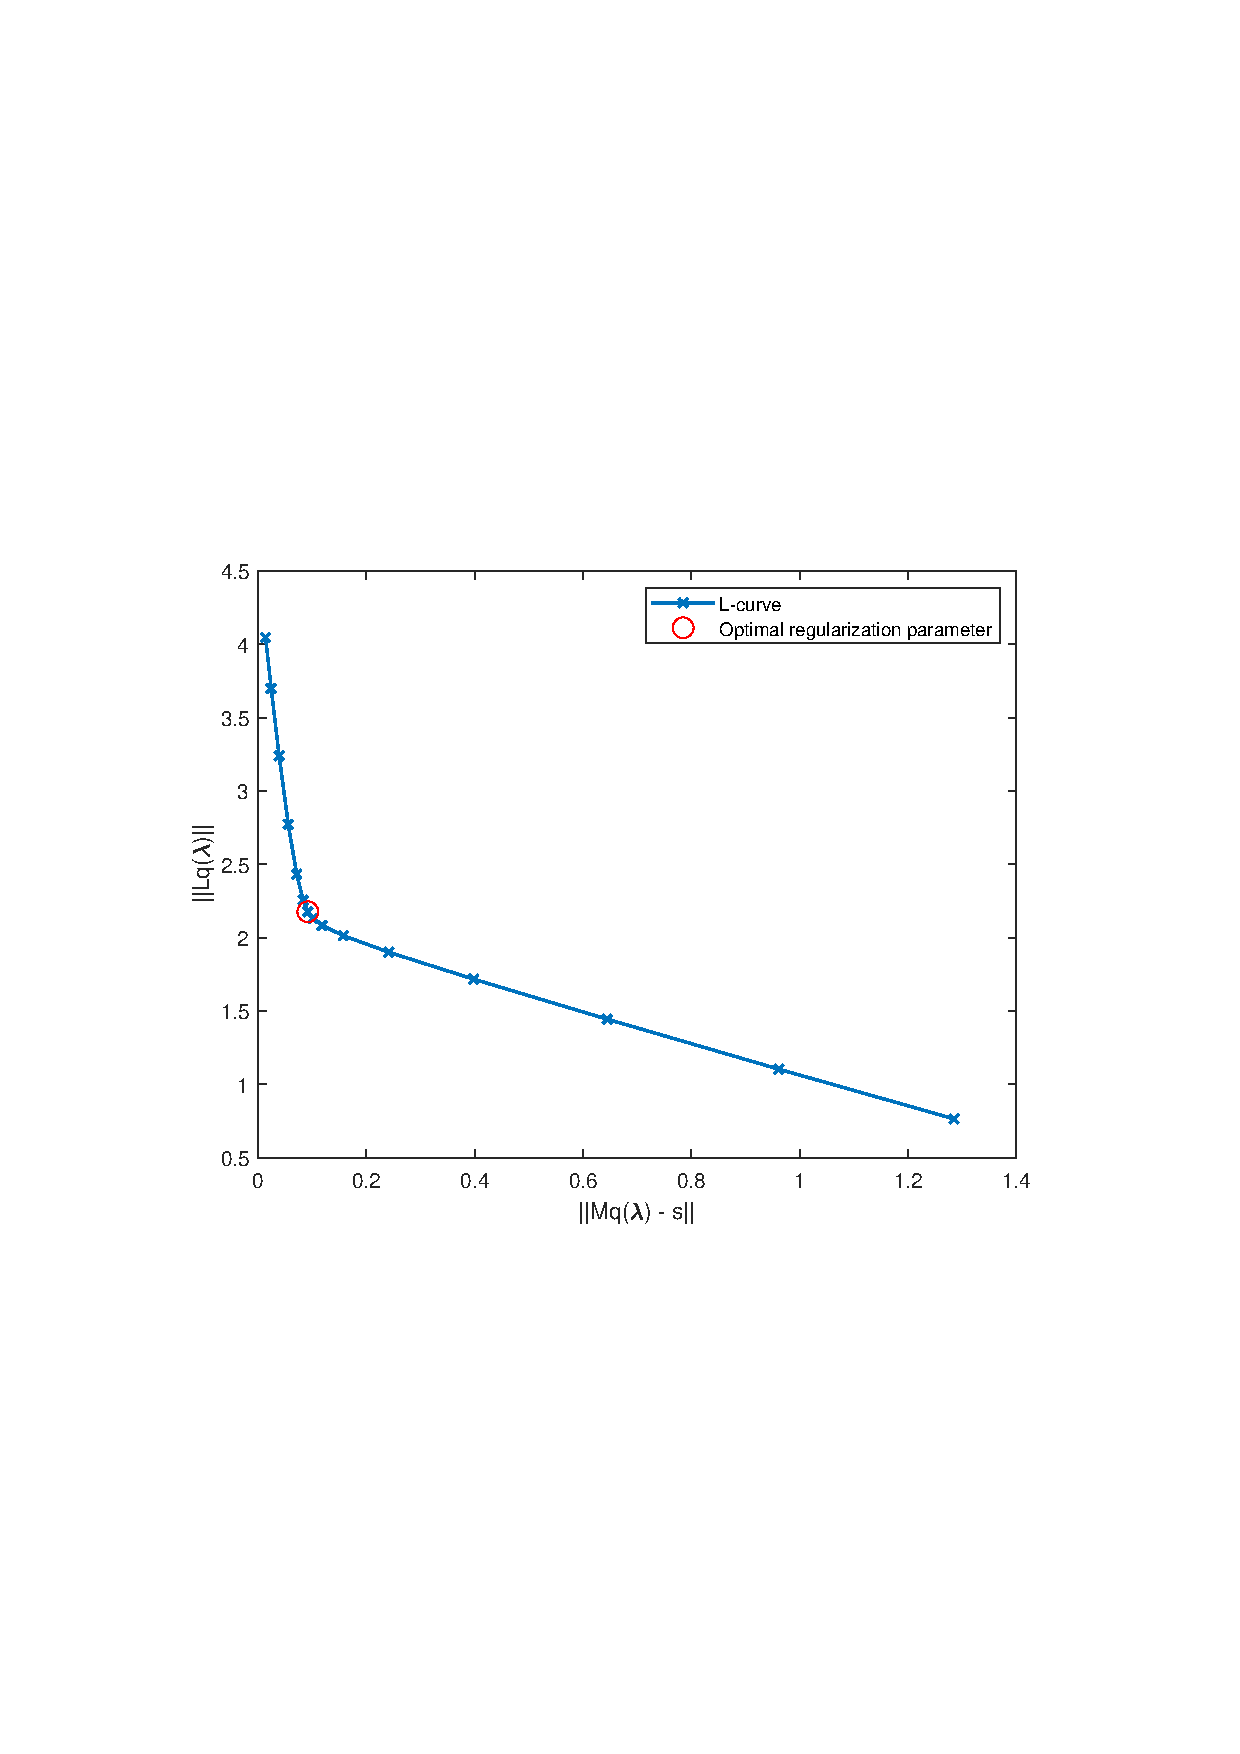
\includegraphics[trim={50 270 100 270},clip]{img/Tikhonov_real.pdf}
    \caption{Typical L-curve scheme with the smallest possible lambda with the most stable value.}
    \label{fig:tikh}
\end{figure}

\begin{lstlisting}
%% Tikhonov Regularization
M = s.orig.added.A;
s_tik = s.noise.added.I_d;
range = 1e-4 * 2.^(0:1:14);
x = zeros(length(range));
y = zeros(length(range));
L = eye(5) + 0.5*randn(5);
q_lam = @(lam) (M'*M+lam*(L'*L))\M'*s_tik;
mq_norm = @(lam) norm(M*q_lam(lam)-s_tik,2);
lq_norm = @(lam) norm(L*q_lam(lam),2);
q_norm = @(lam) norm(q_lam(lam),2);
x = arrayfun(mq_norm,range);
y = arrayfun(lq_norm,range);
dy = [0,diff(y)];
ddy = [0, diff(dy)];
dddy = [0, diff(ddy)];
max_dist = max(dddy);
fig =figure;
plot(x,y,'x-','LineWidth',1.2,'DisplayName','L-curve');
hold on
legend;
xlabel('||Mq(\lambda) - s||');
ylabel('||Lq(\lambda)||');
pos_opt = find(max(dddy)== dddy)+2;
plot(x(pos_opt),y(pos_opt),'ro','MarkerSize',10,'DisplayName',...
'Optimal regularization parameter');
q_lam(x(pos_opt))
print(fig,'fig/Tikhonov.eps','-dpdf');
\end{lstlisting}


